\documentclass[12pt,a4paper]{article}

%%%%%%%%%%%%%%%%%%%%%%%%% packages %%%%%%%%%%%%%%%%%%%%%%%%
\usepackage{amsmath}
\usepackage{amssymb}
\usepackage{amsthm}
\usepackage{amsfonts}
\usepackage{graphicx}
\usepackage[utf8]{inputenc}
\usepackage[english]{babel}
\usepackage[all]{xy}
\usepackage{float}
\usepackage{tikz}
\usepackage{verbatim}
\usepackage[left=2cm,right=2cm,top=2cm,bottom=2cm]{geometry}
\usepackage{hyperref}
\usepackage{caption}
\usepackage{subcaption}
\usepackage{psfrag}
\usepackage{natbib}
%\bibliographystyle{abbrvnat}
\usepackage{booktabs}  
\usepackage[T1]{fontenc}    % use 8-bit T1 fonts
\usepackage{url} 
\usepackage{listings}
\usepackage{xcolor}

\definecolor{codegreen}{rgb}{0,0.6,0}
\definecolor{codegray}{rgb}{0.5,0.5,0.5}
\definecolor{codepurple}{rgb}{0.58,0,0.82}
\definecolor{backcolour}{rgb}{0.95,0.95,0.92}

\lstdefinestyle{mystyle}{
	backgroundcolor=\color{backcolour},   
	commentstyle=\color{codegreen},
	keywordstyle=\color{magenta},
	numberstyle=\tiny\color{codegray},
	stringstyle=\color{codepurple},
	basicstyle=\ttfamily\footnotesize,
	breakatwhitespace=false,         
	breaklines=true,                 
	captionpos=b,                    
	keepspaces=true,                 
	numbers=left,                    
	numbersep=2pt,                  
	showspaces=false,                
	showstringspaces=false,
	showtabs=false,                  
	tabsize=1
}

\lstset{style=mystyle}

\usepackage{color}
\newcommand{\donna}[1]{{\color{red}{#1}}}   
\newcommand{\ignore}[1]{}

%%%%%%%%%%%%%%%%%%%%% students data %%%%%%%%%%%%%%%%%%%%%%%%
\newcommand{\student}{Brian KYANJO }
\newcommand{\course}{Dr. Jodi Mead, Michal Kopera, and Dylan Mikesell}
\newcommand{\assignment}{ Prof. Donna Calhoun}

%%%%%%%%%%%%%%%%%%% using theorem style %%%%%%%%%%%%%%%%%%%%
\newtheorem{thm}{Theorem}
\newtheorem{lem}[thm]{Lemma}
\newtheorem{defn}[thm]{Definition}
\newtheorem{definition}{Definition}[section] 
\newtheorem{theorem}{Theorem}
\newtheorem{exa}[thm]{Example}
\newtheorem{rem}[thm]{Remark}
\newtheorem{coro}[thm]{Corollary}
\newtheorem{quest}{Question}[section]

%%%%%%%%%%%%%%  Shortcut for usual set of numbers  %%%%%%%%%%%

\newcommand{\N}{\mathbb{N}}
\newcommand{\Z}{\mathbb{Z}}
\newcommand{\Q}{\mathbb{Q}}
\newcommand{\R}{\mathbb{R}}
\newcommand{\C}{\mathbb{C}}

%%%%%%%%%%%%%%%%%%%%%%%%%%%%%%%%%%%%%%%%%%%%%%%%%%%%%%%555
\begin{document}
	
	%%%%%%%%%%%%%%%%%%%%%%% title page %%%%%%%%%%%%%%%%%%%%%%%%%%
	\thispagestyle{empty}
	\begin{center}
		\textbf{A Riemann Solver for Wet/Dry Interfaces in Geoclaw \\[0.5cm]
			Synthesis Paper}
		\vspace{.2cm}
	\end{center}
	
	%%%%%%%%%%%%%%%%%%%%% assignment information %%%%%%%%%%%%%%%%
	 
	\rule{17cm}{0.2cm}\\[0.3cm]
	Name: \student \hfill Supervisor: \assignment\\[0.1cm]
	Committee: \course \hfill Date: \today\\
	\rule{17cm}{0.05cm}
	\vspace{.2cm}
	
	\section{Introduction}



	A Riemann Problem is a fundamental problem in conservation laws and is useful in finite volume schemes. It can be defined as a specific initial value problem  (Cauchy) of a partial differential equation (PDE) that consists of conservation equations \eqref{rp0}  combined with piece-wise constant initial data which has a single discontinuity in the domain of interest as shown in equation\eqref{rp1}. 
	\begin{eqnarray}
		q_{t} + f(q)_{x}& =& 0
		\label{rp0}\\
		q(x,0)& =& \begin{cases}
			q_{L}, & \text{if \, $x \le 0,$}\\
			q_{R},& \text{if \, $x > 0,$}\\
			
		\end{cases}  
		\label{rp1}     
	\end{eqnarray}
	where $f(q)_{x} \in \mathbb{R}^{m}$ is a vector of conserved quantities,  $q_{R}$ and $q_{L}$ are two piece-wise constant states separated by a discontinuity. 
	
	\section{Shallow Water Equations (SWE)}
	The SWE are a system of hyperbolic PDEs governing the flow below a pressure surface in a fluid. They arise from the Navier-Stokes equations.  In one dimension, the SWE  can be used to model a fluid in a channel of unit width, taking the vertical velocity negligible, and horizontal velocity roughly constant throughout any cross section of the channel \cite{ge:2008}.  \\
	
	Consider a small-amplitude waves in a one-dimensional fluid channel that is shallow relative to its wavelength. The conservation of momentum equation is written in terms of pressure, $p(x,t) = \frac{1}{2}\rho gh^{2}$, and the height field $h(x,t)$ ($m$), which breaks down into system \eqref{p2}.
	
	\begin{equation}
	\begin{aligned}
		h_{t} + (uh)_x &= 0 \\
		(hu)_t + \left(hu^{2} + \frac{1}{2}\rho gh^{2} \right)_x & = 0 
	\end{aligned}
	\label{p2}
	\end{equation}	
	where $hu$ measures the flow rate of water past a point,  $\rho$ ($kg/m^3$) is the constant density of the incompressible fluid, and $u(x,t)$ ($m/s$) is the horizontal velocity.  We will set $\rho = 1$ here.\\
	
	A very simple set of initial conditions is a single discontinuity at the middle of the channel.  In this case, we set $h$ and $hu$ equal to constants on either side of the channel.  This problem is a classic Riemann Problem, and for the SWE, has an exact solution.  We assume the discontinuity is at $x = 0$. 
	The variation of $h$ and $hu$ on either side of the discontinuity leads the waves in the Riemann problem to move at different speeds creating discontinuities (shocks) or changing regions (rarefactions).  At $x = 0$ and $t = 0$,   the discontinuity is located between the left and right state, so the solution at the left ($q_{l}$)and right($q_{r}$) states are given by: 
	\begin{equation}
		q_{l} = \begin{bmatrix}
			h_{l} \\( hu)_{l}
		\end{bmatrix}  \quad \text{and} \quad q_{r} = \begin{bmatrix}
			h_{r} \\( hu)_{r}
		\end{bmatrix} 
	\label{ic}
	\end{equation}
	As $t$ increases, four distinct regions are created, separated by characteristics. 
	The middle state called the intermediate state($q_{m}$), is generated.  The determination of this state characterizes the Riemann problem and how it connects to other states via waves in each respective characteristic family\cite{ba-le-mi-ro:2003}.  This can only hold if the connection wave speeds satisfy the Lax entropy condition. Figure \ref{fig:x-tplane} shows a wave combination of a centered rarefaction  and shock wave from the first and second characteristic family respectively.
	
	\begin{figure}[H]
		\centering
		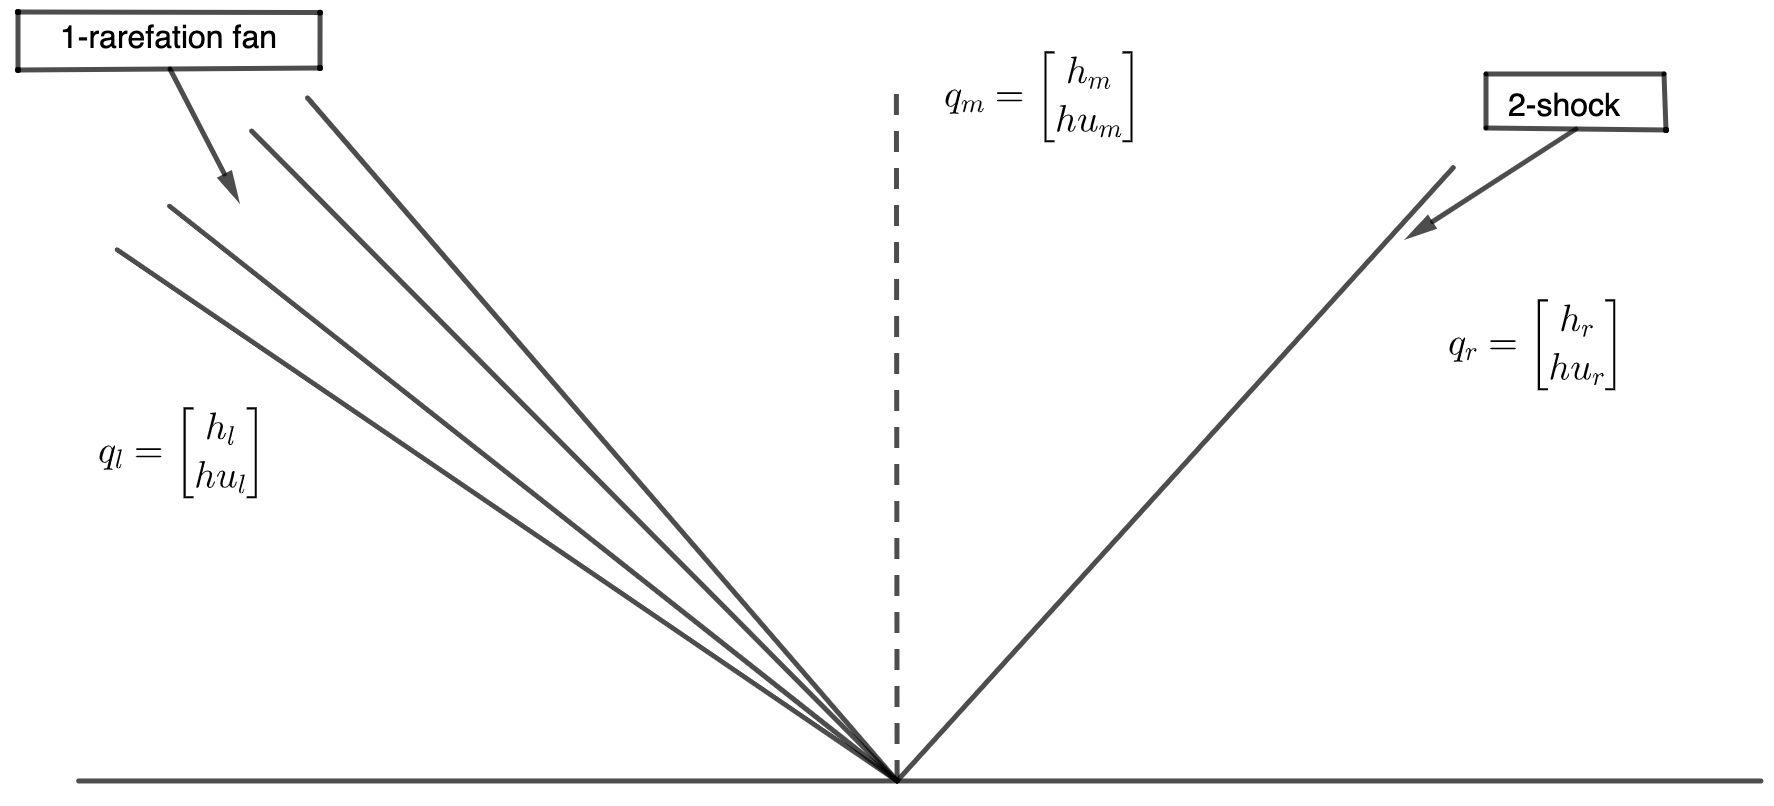
\includegraphics[width=0.5\linewidth]{images/geo1}
		\caption{ x-t plane showing the connection of states, 1-rarefaction fan, and the 2-shock.}
		\label{fig:x-tplane}
	\end{figure}
	
	The intermediate state is obtained by solving the Riemann problem using the exact or  approximate method. Approximate methods are widely used due to their cheap computational cost compared to the exact solvers.
	
	
	\subsection{Exact Riemann Solver for two-shock SWE}
	The states in \ref{fig:x-tplane} are separated by either {\em shocks} or {\em rarefactions}. General left and right states will be connected by a combination of the two (either two shocks, two rarefactions, or one of each).  We describe how to determine if two states are connected by a shock.  We refer the reader to \cite{leveque2002finite} for other cases. 

	We can obtain an exact solution to the Riemann Problem for the SWE as follows. 
	The shock speed, $s(t)$,  from the shock wave as the solution emerges is determined from the Rankine-Hugoniot jump condition given by equation \eqref{e1}  which must be satisfied across any shock wave.  If $q_l$ and $q_r$ are connected by a shock, the Rankine Hugoniot conditions will be satisfied. 
	\begin{equation}
	\begin{aligned}
		s_1(q_{m} - q_{l}) & = f(q_{m}) - f(q_{l}) \\
		s_2(q_{r} - q_{m}) & = f(q_{r}) - f(q_{m})
	\end{aligned}
	\label{e1}
	\end{equation}
	 By applying condition  \eqref{e1} to shallow water equations \eqref{p2}  creates a system of four equations \eqref{ee2} that must be satisfied simultaneously. 
	 
	 	\begin{equation}
	 	\begin{aligned}
	 		s_1(h_{m} - h_{l}) & = hu_{m} - hu_{l} \\
	 		s_1(hu_{m} - hu_{l})  &= hu_{m}^{2} - hu_{l}^{2} + \frac{1}{2}g(h_{m}^{2} - h_{l}^2)\\
	 		s_2(h_{r} - h_{m})  &=  hu_{r} - hu_{m}\\
	 		s_1(hu_{r} - hu_{m})  &= hu_{r}^{2} - hu_{m}^{2} + \frac{1}{2}g(h_{r}^{2} - h_{m}^2)
	 	\end{aligned}
	 	\label{ee2}
	 \end{equation}
 Since the $(h_l,u_l)$ and $(h_r,u_r)$ are fixed, we find all states: $(h_m,u_m)$  and their corresponding speeds: $s_1$ and $s_2$ that satisfy system  \eqref{ee2}. We have four equations and four unknowns, which gives a two parameter family of solutions: one-shock and two-shock. Using $h_l$ and $h_r$ as parameters, corresponding $u_l,u_r,s_1, $and $s_2$ are determined for each $h_l$ and $h_r$. And then a graph of $hu$ against $h$ is plotted that gives the curves in fig.~\ref{fig:hl}. The point of intersection between the {\em 1-shock (blue)} and  {\em2-shock (orange)} physical solutions is the intermediate state $q_m$. The dotted curves represent unphysical solution.
  
	\begin{figure}[H]
		\centering
		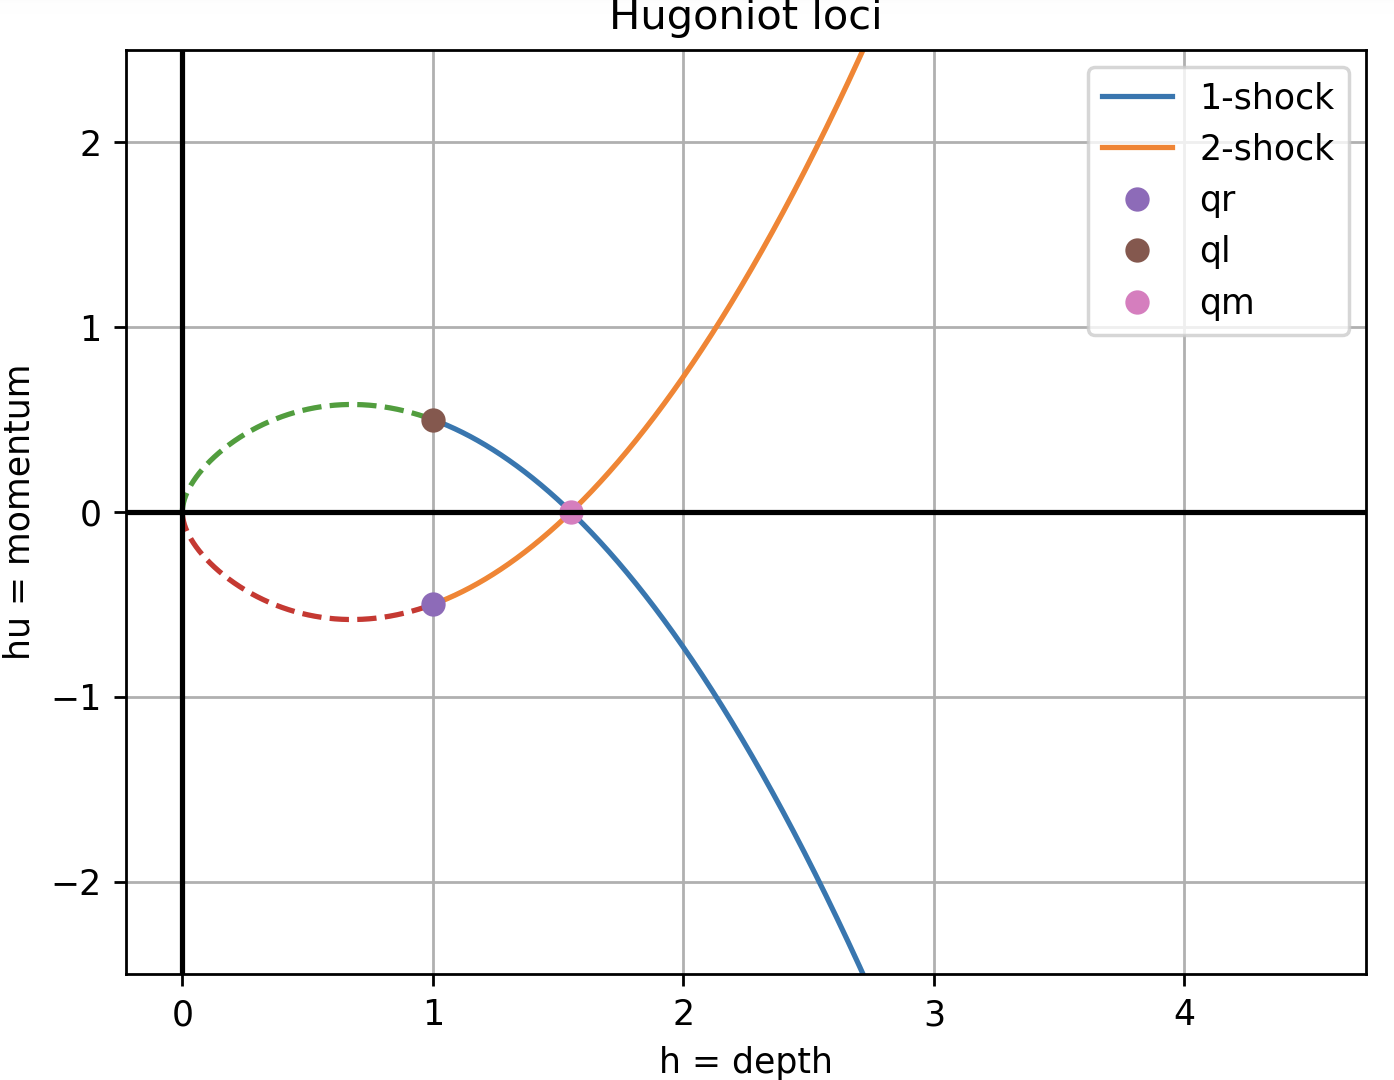
\includegraphics[width=0.5\linewidth]{images/hl}
		\caption{Shows curves that represent all states connected to $q_l$ and all states connected to $q_r$ via a {\em 2-shock} and {\em 1-shock} respectively.  Equations \eqref{e3} and \eqref{e4} are solved to produce the curves.}
		\label{fig:hl}
	\end{figure}

	Consider a general Riemann problem whose known solution consists of two shocks with initial data \eqref{ic}. This problem can be solved by finding the state $q_m$ that can be connected to $q_l$ by a {\em 1-shock} and simultaneously connects to $q_r$ by a {\em 2-shock}. The point $q_m$ lies on the  curve \eqref{e3} of points  through  point $q_r$  that connects to $q_r$ by a {\em 2-shock}.

	\begin{equation}
		u_{m} = u_{r} + (h_{m} - h_{r})\sqrt{\frac{g}{2}\left(\frac{1}{h_m} + \frac{1}{h_r} \right)}
		\label{e3}
	\end{equation}
	Likewise, the state($q_m$), must also lie on the Hugonoit locus (equation \eqref{e4}) of the 1-shock wave passing through $q_l$
	\begin{equation}
		u_{m} = u_{l} - (h_{m} - h_{l})\sqrt{\frac{g}{2}\left(\frac{1}{h_m} + \frac{1}{h_l} \right)}
		\label{e4}
	\end{equation}
	Equations \eqref{e3} and \eqref{e4} form a system of two equations with two unknowns ($h_m$ and $u_m$) that are equated since the left-hand sides of both equations are equal. A non linear equation that consist of only one unknown $h_m$ is formed and solved using an iterative method such as Newton method to obtain a desired intemediate state in the Riemann solution.\\

   As an example, consider athe SWE Riemann problem with $h_l = h_r = 1, u_l = 0.5, $ and $u_r = -0.5$. These initial values are used by the netwon solver to solve equations \eqref{e3} and \eqref{e4} to produce $h_{m} = 1.554$. The shock speeds ($s_l$ and $s_r$) in each region are different due to different wave characteristics, we use this concept to loop through all interfaces and determine $h$ and $hu$ in each region as shown in the code \ref{pp} . At each interface $h$ and $hu$ are stored into $q_1$ and $q_2$ as hieght and momentum solutions. According to Lax entropy conditions, a  {\em 1-shock} that physically connects $q_l$ to $q_m$ is obatined if $h_m>h_l$, and similarly a {\em 2-shock} wave that physically connects $q_m$ to $q_r$ requires $h_m>h_r$ \cite{le-ge-be:2011}.
   
\begin{small}
	\begin{lstlisting}[language=Python, caption=Python code describing how the two shock case solution is obtained after the first time step.,label = pp]
for i in range(len(x)):
		if 0.5*(sl(hl,ql,g) + sl(hm,qm,g))*t > x[i] : # left to middle state
				h = hl
				u = ul
				hu = h*u   	
		elif sl(hm,qm,g)*t < x[i] and x[i]<t*sr(hm,qr,g): # middle state
				h = hm
				u = um
				hu = h*u
		else:     # middle to right state
				h = hr
				u = ur
				hu = h*u
		q1[i] = h
		q2[i] = hu
\end{lstlisting}
\end{small}

The height field solution $q_1$ obtained from the code \ref{pp} above is ploted in fig.~\ref{fig:2-shock}. The plot depicts the left region being connected to the middle region via a {\em 1-shock } wave and the middle  being connected to the right region via a a {\em 2-shock } wave.

	\begin{figure}[H]
		\centering
		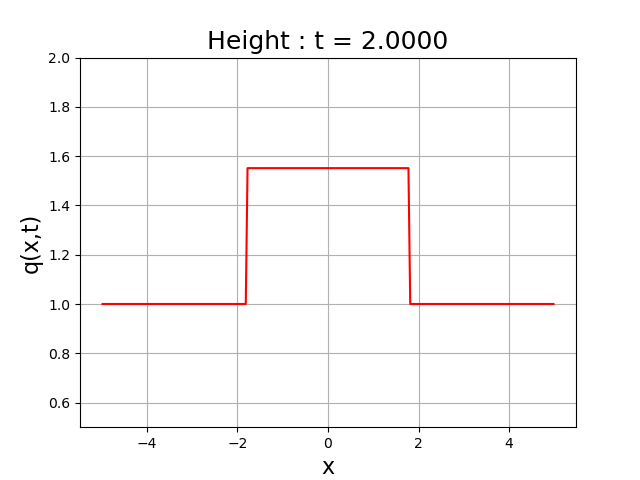
\includegraphics[width=0.5\linewidth]{images/2-shock}
		\caption{Shows all-shock Riemann exact solution }
		\label{fig:2-shock}
	\end{figure}
	

	\section{Finite volume discretization}
	Consider a one dimensional (1D) conservation law  (equation \eqref{fvm0}),  where $q$ is the measure of conserved quantity density and $f(q)$ is a flux function.
	\begin{equation}
		q_{t}(x,t) + f(q(x,t))_{x} = 0
		\label{fvm0}
	\end{equation}	
	  In finite volume methods (FVM), the domain is broken down into grid cells. Consider $C_{i} = (x_{i-\frac{1}{2}},x_{i+\frac{1}{2}})$ to be the $i^{th}$ grid cell, the average value over the $i^{th}$ interval at time $t^{n}$ is numerically approximated by $Q_{i}^{n}$ in equation \eqref{wpa0}.
	
	\begin{equation}
		Q_{i}^{n} \approx \dfrac{1}{\Delta x} \int_{C_{i}}q(x,t^{n})dx
		\label{wpa0}
	\end{equation}
	   where $\Delta t = (t^{n+1} - t^{n})$ and  $\Delta x = (x_{i+\frac{1}{2}} - x_{i-\frac{1}{2}})$ is the cell length. A discontinuity in $q$ violates the PDE in the classical sense and only holds for the integral conservation law (fundamental equation \eqref{fvm1}). Therefore at grid points near discontinuities where PDEs don't hold, all classical finite difference methods breakdown, resorting to FVM which are based on \eqref{fvm1}. 	
	\begin{equation}
		\frac{d}{dt} \int_{c_{i}} q(x,t)dx = f(q(x_{i-\frac{1}{2}},t)) -  f(q(x_{i+\frac{1}{2}},t))
		\label{fvm1}
	\end{equation}	
	The approximate  total integral of $q$ over each grid cell is evaluated and updated at every time step by the grid cell edge fluxes. The determined numerical flux functions evaluate the  cell averages over a certain volume, which are used to approximate the solutions within the cells, using equation \eqref{cellupdate}.
	
	\begin{equation}
		Q_{i}^{n+1} = Q_{i}^{n} - \frac{\Delta t}{\Delta x} (F_{i+\frac{1}{2}}^{n} - F_{i-\frac{1}{2}}^{n})
		\label{cellupdate}
	\end{equation}	
	  where $F_{i+\frac{1}{2}}^{n} $ is the average flux approximation along $x=x_{i-\frac{1}{2}}$.
	The Riemann problem is a fundamental tool in the evolution of FVM. Taking two neighbouring grid cells: $Q_{i-1} = q_{L}$ and $Q_{i} = q_{R}$ to be cell averages, this information is used by the exact Riemann solver to compute numerical fluxes ( $F_{i-\frac{1}{2}}^{n} = \mathcal{F}(Q_{i-1} , Q_{i} )$), that are used to update the cell average at each time step \cite{ba-le-mi-ro:2003}. Then equation \eqref{cellupdate} becomes:
	
	\begin{equation}
		Q_{i}^{n+1} = Q_{i}^{n} - \frac{\Delta t}{\Delta x} \left[ \mathcal{F}(Q_{i} , Q_{i+1} ) - \mathcal{F}(Q_{i-1} , Q_{i} ) \right]
		\label{cellupdat}
	\end{equation}
	where $\mathcal{F}$ is some numerical flux function.\\
	
	\section{Wave Propagation Algorithm (WPA)}
	  Equation \eqref{cellupdate}, can be reformulated as a first order wave propagation method by decomposing flux at the cell averages into fluctuations ($\mathcal{A^{+}}\Delta 	Q_{i-\frac{1}{2}}^{n}$ and  $\mathcal{A^{-}}Q_{i+\frac{1}{2}}^{n}$) as shown in equations \eqref{ap} and \eqref{am}. 
	
	\begin{eqnarray}
		\mathcal{A^{+}}\Delta Q_{i-\frac{1}{2}}^{n} = f(Q_{i}) - f(Q_{i-\frac{1}{2}}^{*})
		\label{ap}\\
		\mathcal{A^{-}}\Delta Q_{i+\frac{1}{2}}^{n} = f(Q_{i+\frac{1}{2}}^{*}) - f(Q_{i}) 
		\label{am}
	\end{eqnarray}	
	  where  $\mathcal{A^{+}}\Delta 	Q_{i-\frac{1}{2}}^{n}$ and  $\mathcal{A^{-}}Q_{i+\frac{1}{2}}^{n}$ are the net updating contributions from the rightward and leftward moving waves into the grid cell $C_{i}$  from the right and left interface respectively,  $Q_{i-\frac{1}{2}}^{*}$ is the intermediate cell average determined by the exact Riemann solver at $x_{i-\frac{1}{2}}$, and $ f(Q_{i-\frac{1}{2}}^{*})$ is numerical flux at $Q_{i-\frac{1}{2}}^{*}$. Combining equations \eqref{ap} and \eqref{am}, the  first order 1D  wave propagation method is given by equation \eqref{wpa0}.
	
	\begin{equation}
		Q_{i}^{n+1} =  Q_{i}^{n} - \frac{\Delta t}{\Delta x}(\mathcal{A^{+}}\Delta 	Q_{i-\frac{1}{2}}^{n} + \mathcal{A^{-}}Q_{i+\frac{1}{2}}^{n})
		\label{wpa0}
	\end{equation}
	\label{section:my}
	The general conservation law in \eqref{fvm0} can be written in {\em quasi-linear form}
	as
	\begin{equation}
		q_{t} + f'(q)q_{x} = 0
		\label{wpa3}
	\end{equation}
	where  $f'(q) \in \mathbb{R}^{m\times m}$  flux Jacobian matrix.  Consider a Riemann problem for the system  \eqref{wpa3} with initial data 
	
	\begin{equation}
		q(x,t^n)  = \begin{cases}
			Q_{i-1}^{n}  & \text{if} \quad  x < x_{i-\frac{1}{2}}\\
			Q_{i}^{n} & \text{if} \quad x > x_{i-\frac{1}{2}}\\
		\end{cases}    
		\label{w4}   
	\end{equation}
	The initial data (equation \eqref{w4}), is used by the exact Riemann solver to generate an intermediate state ($q_m = (h_m, hu_m)^T$), which is used to evaluate the eigenvalues ($\lambda_{i-1/2}$) and eigenvectors ($r_{i-1/2}$) at $x = x_{i-\frac{1}{2}}$. The $p^{th}$ wave at interface $i-1/2$ is given by $\mathcal W^p_{i-1/2} \equiv \alpha_{i-\frac{1}{2}} r^p_{i-\frac{1}{2}}$ with speeds $s^p_{i-1/2} = \lambda^p_{i-1/2}$. where $ \alpha_{i-\frac{1}{2}}$ depicts the coefficients of the the eigenvectors.  Waves and speeds are obtained as an eigenvector decomposition of the jump in $Q_i$ at the interface $i-\frac{1}{2}$.  This decomposition takes the form
	 
	\begin{equation}
		Q_{i} -  Q_{i-1} = \sum_{p=1}^{m}  \alpha_{i-\frac{1}{2}} r_{i-\frac{1}{2}}
		\label{wpa19}
	\end{equation}
	  The wave speed $s_{i-\frac{1}{2}}^{p}$ associated with the vector $r_{i-\frac{1}{2}}^{p}$, are preselected basing on the characteristic structure of the initial Riemann data \cite{ge:2008}. Therefore the fluctuations $\mathcal{A^{+}}\Delta Q_{i-\frac{1}{2}}^{n}$  and $\mathcal{A^{-}}\Delta Q_{i-\frac{1}{2}}^{n} $ are defined by equations \eqref{f0} and \eqref{f1}:
	
	\begin{eqnarray}
		\mathcal{A^{-}}\Delta Q_{i-\frac{1}{2}}^{n} = \sum_{\{ p:s_{i-\frac{1}{2}}^{p}<0\}} s_{i-\frac{1}{2}}^{p} \mathcal{W}_{i-\frac{1}{2}}^{p}
		\label{f0}\\
		\mathcal{A^{+}}\Delta Q_{i-\frac{1}{2}}^{n} =\sum_{\{ p:s_{i-\frac{1}{2}}^{p}>0\}} s_{i-\frac{1}{2}}^{p} \mathcal{W}_{i-\frac{1}{2}}^{p}
		\label{f1}
	\end{eqnarray}
	  In a standard  conservative case (\eqref{fvm0}), the sum of the left-going and right-going fluctuations should satisfy:
	
	\begin{equation}
		\mathcal{A^{+}}\Delta 	Q_{i-\frac{1}{2}}^{n} + \mathcal{A^{-}}Q_{i+\frac{1}{2}}^{n} = f(Q_{i}) - f(Q_{i-1})
	\end{equation}
	%\donna{Be prepared to explain why this must be true.}
	The second order accuracy is obtained by taking the correction terms into account as shown described in equation \eqref{wpa2}
	
	\begin{equation}
		Q_{i}^{n+1} =  Q_{i}^{n} - \frac{\Delta t}{\Delta x}(\mathcal{A^{+}}\Delta 	Q_{i-\frac{1}{2}}^{n} + \mathcal{A^{-}}Q_{i+\frac{1}{2}}^{n}) -  \frac{\Delta t}{\Delta x} (\tilde{F}_{i+\frac{1}{2}}^{n} - \tilde{F}_{i-\frac{1}{2}}^{n} )
		\label{wpa2}
	\end{equation}
	  where $\tilde{F}_{i-\frac{1}{2}}^{n} $ are second order correction terms determined by the waves and speeds in the Riemann problems after approximating the average flux along  $x = x_{i - \frac{1}{2}}$:
	
	\begin{equation}
		\tilde{F}_{i-\frac{1}{2}}^{n} = \frac{1}{2} \sum_{p=1}^{m}  |s_{i- \frac{1}{2}}^{p}| \left( 1 - \frac{\Delta t}{\Delta x} |s_{i- \frac{1}{2}}^{p}|\right) \tilde{\mathcal{W}}_{i-\frac{1}{2}}^{p} 
		\label{wpa13}
	\end{equation}
	  Here $\tilde{\mathcal{W}}_{i-\frac{1}{2}}^{p} $ depicts a limited version of the wave $\mathcal{W}_{i-\frac{1}{2}}^{p} $, which is obtained after a comparison between $\mathcal{W}_{i-\frac{1}{2}}^{p} $ and $\mathcal{W}_{i-\frac{3}{2}}^{p} $ when $s^{p} >0$.\\
	
	\subsection{WPA for the Shallow Water Equations}
	
	 	The combination of equations in system \eqref{p2}, forms a system of one-dimensional SWEs given by equation \eqref{p3}
	
	\begin{eqnarray}
		\begin{bmatrix} h \\ hu \end{bmatrix}_t + \begin{bmatrix} uh \\ hu^{2} + \frac{1}{2} gh^{2} \end{bmatrix}_x  = 0 
		\label{p3}
	\end{eqnarray}
	Equation \eqref{p3} can be written as a quasi-linear system as shown in equation \eqref{p4}:
	
	\begin{equation}
		\begin{bmatrix} h \\ hu \end{bmatrix}_t + 
		\begin{bmatrix} 0 &  1 \\ -u^{2} + gh & 2u \end{bmatrix} 
		\begin{bmatrix} h \\ hu \end{bmatrix}_x =  
		\begin{bmatrix} 0 \\ 0 \end{bmatrix}
		\label{p4}
	\end{equation}
	where the flux Jacobian matrix $f'(q)$ is given by 
	\begin{equation}
	f'(q) = \begin{bmatrix} 0 &  1 \\ -u^{2} + gh & 2u \end{bmatrix} 
	\end{equation}
	The non linear problem (equation \eqref{fvm0}), can be replaced by a linearized problem defined locally at each cell interface \cite{le-ge-be:2011},
	\begin{equation}
		\hat{q}_t + \hat{A}_{i-\frac{1}{2}}  \hat{q}_x  = 0
		\label{n2}
	\end{equation}
	  where $2 \times 2$ matrix $\hat{A}_{i-\frac{1}{2}} $ (equation \eqref{n3}) is selected to be an approximation of $f^{\prime}(q)$ that is valid in the neighbourhood of the intial data $Q_{i-1}$ and $Q_{i}$.
	\begin{equation}
		\hat{A}_{i-\frac{1}{2}} =  \begin{bmatrix} 0 &  1 \\ -\hat{u}^{2} + g\bar{h} & 2\hat{u} \end{bmatrix} 
		\label{n3}
	\end{equation}
	  where $\bar{h} = \frac{1}{2}(h_{i-1} + h_{i})$ is the average between end points $h_{i-1}$ and $h_{i}$, $g$ is the acceleration due to gravity, and $\hat{u} = (\sqrt{h_{i-1} }u_{i-1} + \sqrt{h_i}u_i)/(\sqrt{h_{i-1}} + \sqrt{h_i})$ is the Roe average. Since $\hat{A}_{i-\frac{1}{2}} $ is a real diagonalizable Jacobian matrix evaluated at $\hat{q} = (\bar{h},\bar{h}\hat{u})$, then its eigenvalues ($\hat{\lambda}$) and eigenvectors ($\hat{r}$) are given by equations  \eqref{eg} and \eqref{vec} respectively.
	\begin{equation}
		\hat{\lambda}^1 = \hat{u} - \hat{c}, \qquad 	\hat{\lambda}^2 = \hat{u} + \hat{c}
		\label{eg}
	\end{equation}
	
\begin{equation}
\hat{r}^1 =  \begin{bmatrix} 1 \\ 	\hat{\lambda}^1 \end{bmatrix}, \qquad 	\hat{r}^2 =  
\begin{bmatrix} 1 \\ 	\hat{\lambda}^2 \end{bmatrix}
\label{vec}
\end{equation}
where $\hat{c} = \sqrt{gh}$, the approximate Riemann solver is used to decompose the vector  $ \delta \equiv Q_{i} - Q_{i-1}$ into two waves: $\alpha_{i-\frac{1}{2}}^{1} \hat{r}^1$ and $\alpha_{i-\frac{1}{2}}^{1} \hat{r}^2$ as 
\begin{equation}
Q_{i} - Q_{i-1} = \alpha_{i-\frac{1}{2}}^{1} \hat{r}^1 + \alpha_{i-\frac{1}{2}}^{1} \hat{r}^2 \equiv \mathcal{W}_{i-\frac{1}{2}}^{1} + \mathcal{W}_{i-\frac{1}{2}}^{2}
\end{equation}
where the coefficients $\alpha_{i-\frac{1}{2}}^{1}$ are given by:
\begin{eqnarray}
\alpha_{i-\frac{1}{2}}^{1} &=& \frac{(\hat{u} + \hat{c})\delta^{1} - \delta^2}{2\hat{c}}\\
\alpha_{i-\frac{1}{2}}^{2} &=& \frac{-(\hat{u} - \hat{c})\delta^{1} + \delta^2}{2\hat{c}}
\end{eqnarray}
	
\section{Limiters}
Accuracy of smooth solutions are obtained by advancing first order methods to second order accurate, but these still fail at the neighbourhood of discontinuities, where oscillations (noise) are created as shown in fig.~\ref{fig:2nd}. Limiters use the characteristics of the solution at such regions to filter out the oscillations eliminating the phase error hence increasing accuracy as depicted in fig.~\ref{fig:2lim}. The second order correction terms are computed basing on several different families of waves produced by the Riemann solution, the superposition of such waves make limiting process very difficult \cite{ge:2011} .  Since in some regions, some waves may be discontinuous while others are smooth, therefore different limiter types handle this process in a different way, making some limiters to perform better than others depending on the method they are applied too \cite{be-ge-le-ma:2011}.\\
	
	  The Dispersive nature of some methods may produce oscillations even in smooth solutions. During the simulations we focused on using only  four high-resolution limiters: minmod, superbee, MC, and van Leer.
	\begin{eqnarray}
		\text{minmod} :~ \phi(\theta) &=& \text{minmod}(1,\theta)\\
		\text{MC} : ~ \phi(\theta) &=& \text{max} \left(0,\frac{\text{min}(1 + \theta)}{2},2,2\theta \right)\\
		\text{superbee}: ~ \phi(\theta) &=& \text{max}(0,\text{min}(1,2\theta),\text{min}(2,\theta))\\
		\text{van Leer} : ~ \phi(\theta) &=& \frac{\theta + |\theta|}{1 + |\theta|}
	\end{eqnarray}
	  where $\phi(\theta)$ is a limiter function. Each limiter behaved differently in phasing out oscillations, even though the simple limiter (minmod), performed better  in filtering out the noise near the 2-shock for the flux formulation method as shown in fig.~\ref*{fig:2lim}, since its a slope limiter that lies along the lower boundary of the Sweby region in the $\theta$-$\phi$  plane. Full second order accuracy is obatined for MC if the function $\phi$ is smooth near $\theta=1$. The van Leer is a smoother version of MC, and the superbee lies along the upper boundary of the Sweby region and it did not perform well because it gives much too compression  \cite{ma-ah-be-ca-ge-ha-ke-le-le:2016}.\\
	\section{Numerical Examples}
	
	Figures \ref{fig:1st} and  \ref{fig:2nd}, represents two plots: first  and second order correction (without limiters) obtained from simulation of WPA flux formulation and WPA using the Roe solver combined with the exact Riemann solver. The dam break problem is solved using both flux formulation and  Roe solver, and  solutions are validated against the exact Riemann solver solution as shown in the two figures. For the first order solution both methods coincide even though they tend to flatten at both edges of the 1-rarefaction fan and the 2-shock. On applying the second order correction in  \ref{fig:2nd}, the solutions at edges of each region tend to converge more to the exact solution, however more noise is exhibited at the beginning and end of the intermediate region, and this can be solved by applying limiters to the approximate solutions as shown in fig.~\ref{fig:2lim}. \\
	
	Figure.~\ref{fig:2lim} depicts the filtration of oscillations around the 1-rarefaction fan and 2-shock discontinuity regions in fig.~\ref{fig:2nd} after application of limiters at the final time. It's seen that the height field solution exhibits a smooth through out the the entire simulation even at jumps in the solution compared to  fig.~\ref{fig:2nd}. This improved the accuracy of the second order method, simulating well the boundaries of several regions without noise.
	\begin{figure}[H]
		\begin{subfigure}[b]{0.5\textwidth}
			\centering
			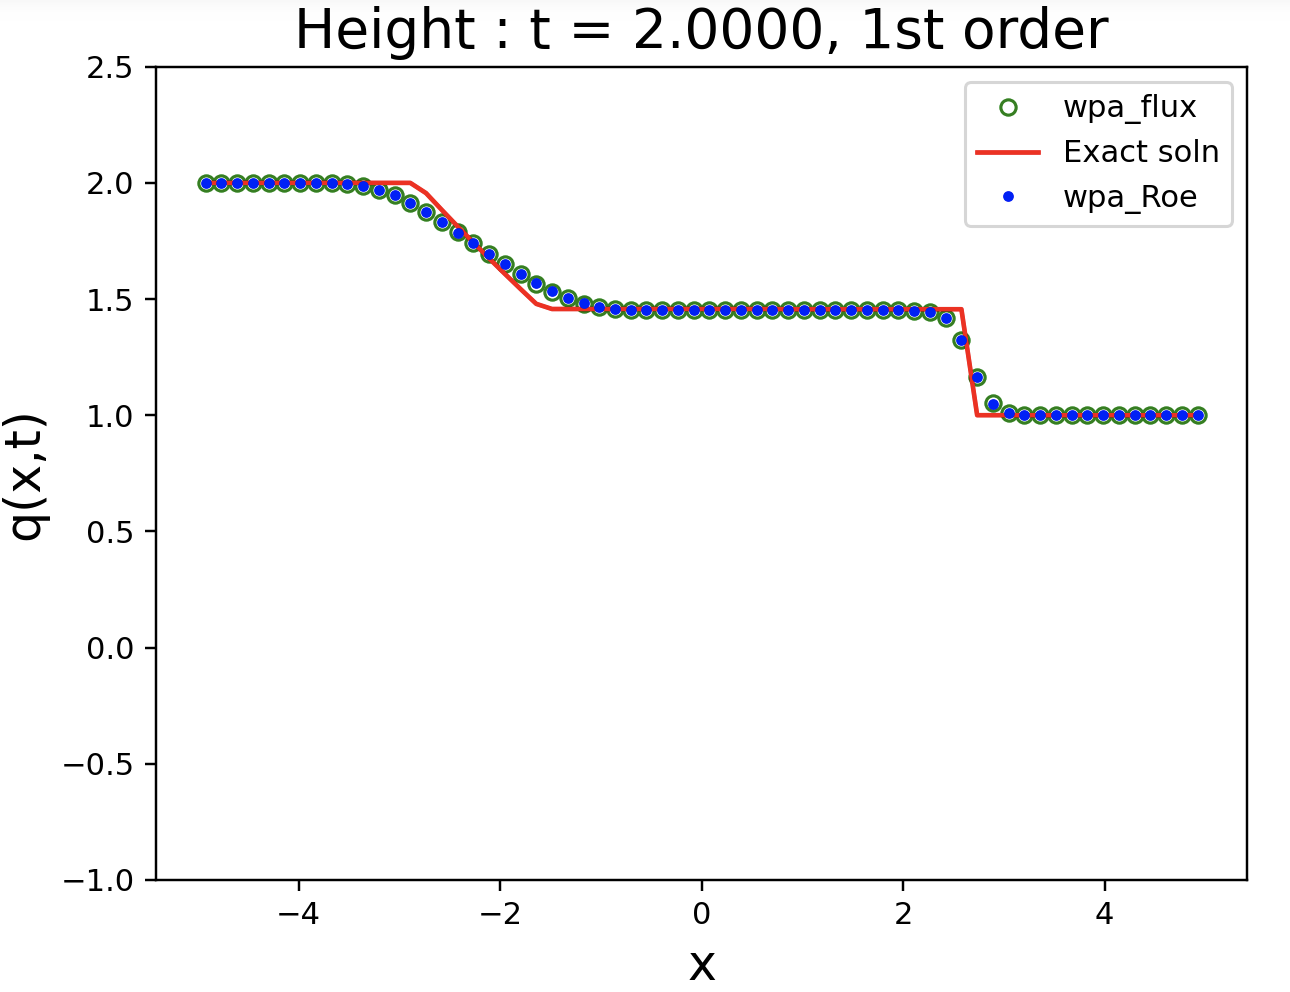
\includegraphics[width=1.0\linewidth]{images/1st}
			\caption{}
			\label{fig:1st}
		\end{subfigure}
		%
		\begin{subfigure}[b]{0.5\textwidth}
			\centering
			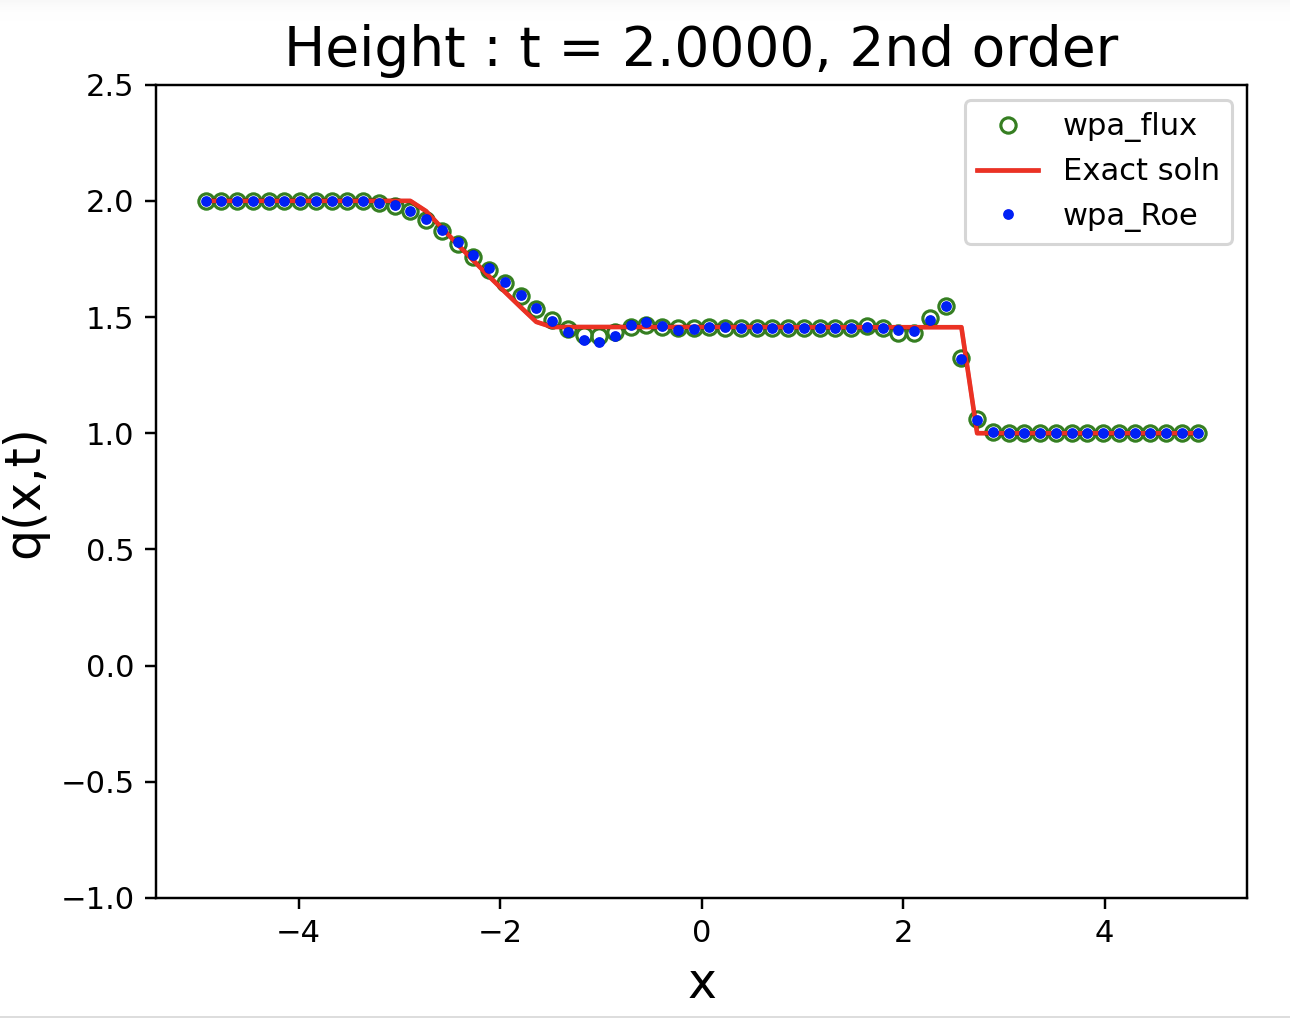
\includegraphics[width=1.0\linewidth]{images/2nd}
			\caption{}
			\label{fig:2nd}
		\end{subfigure}
		\caption{(a) and (b) respectively show height field at the final time step for both first and second order correction without limiters using 64 space points. }
	\end{figure}

	\begin{figure}[H]
		\centering
		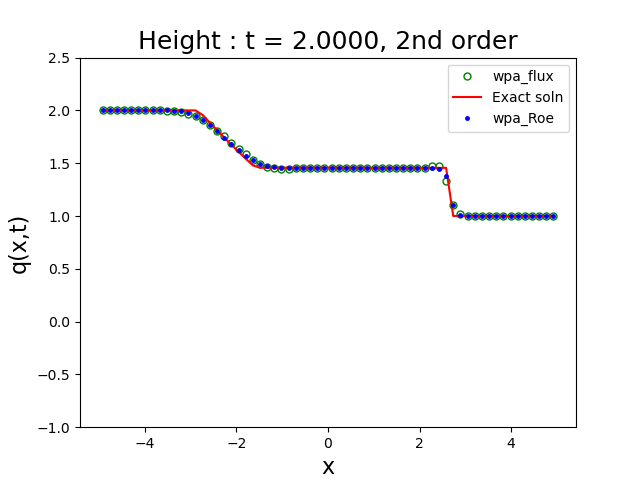
\includegraphics[width=0.6\linewidth]{images/2lim}
		\caption{Shows the height field at the final time step of second order correction with limiter using 64 space points.}
		\label{fig:2lim}
	\end{figure}
	
	\subsection{ Bathymetric source terms}
	Equation \eqref{p2}, can be extended to balance equations by introducing a bathymetric source term as shown in equation \eqref{bst}. This is done by discretising the source term to generate values $-gh_{i-\frac{1}{2}}B^{\prime}(x_{i-\frac{1}{2}})$ at  cell interfaces  $x = x_{i-\frac{1}{2}}$. This approach is very useful, because the discrepancy caused due to the failure of the flux gradient to counterbalance the source term in a near steady state solution is decomposed into propagating waves  making the approach more robust than the quasi-steady WPA \cite{ba-le-mi-ro:2003}.
	\begin{equation}
		\begin{aligned}
			h_{t} + (uh)_x &= 0 \\
		(hu)_t + \left(hu^{2} + \frac{1}{2}gh^{2} \right)_x =& -ghB^{\prime}(x)
		\label{bst}
		\end{aligned}
	\end{equation}
	where $B(x)$ represents bottom elevation. \\
	
	%\subsection{ Introduce fwaves to handle stationery states}
	  The fwaves are introduced to handle the stationery states and also solve accurately  the quasi-steady problems in which the objective is to obtain propagation due to small amplitude perturbations. The standard WPA (\ref{section:my}) is conservative if and only if equation \eqref{con} is satisfied, but the flux-based wave decomposition yields a more flexible algorithm that is conservative even when equation\eqref{con} is not satisfied. And works perfect even for problems in which the Roe average is not easily computed \cite{ba-le-mi-ro:2003}.
	
	\begin{equation}
		A_{i-\frac{1}{2}} (Q_{i} - Q_{i-1}) = f(Q_i) - f(Q_{i-1})
		\label{con}
	\end{equation}
	
	  The flux difference $ f(Q_i) - f(Q_{i-1})$ is directly decomposed as  a linear combination of the eigenvectors $r_{i-\frac{1}{2}}$ as shown in equation \eqref{fw}
	
	\begin{equation}
		f(Q_{i}) - f(Q_{i-1})  - \Delta x \psi_{i-\frac{1}{2}} = \sum_{p=1}^{m} \beta_{i-\frac{1}{2}} ^{p} r_{i-\frac{1}{2}}^{p}  \equiv \sum_{p=1}^{m} \mathcal{Z}_{i-\frac{1}{2}}^{p} 
		\label{fw}
	\end{equation}
	where
	
	\begin{equation}
		\beta_{i-\frac{1}{2}} = R_{i-\frac{1}{2}}^{-1} (f(Q_{i}) - f(Q_{i-1}))  - \Delta x \psi_{i-\frac{1}{2}}
		\label{fw1}
	\end{equation}
	
	  The vectors $\mathcal{Z}^{p} = \beta^{p} r^p$ are called the fwaves, as they are similar to the waves $\mathcal{W}^p$ though they carry flux increments rather than $q$ increments. The standard WPA (\ref{section:my}) first and second order corrections have been advanced to capture the flux based wave decomposition by changing equations \eqref{wpa19} and  \eqref{wpa13}  to  \eqref{fw1} and \eqref{fw2} respectively.
	
	\begin{equation}
		\tilde{F}_{i-\frac{1}{2}}^{n} = \frac{1}{2} \sum_{p=1}^{m}  \text{sgn}(s_{i- \frac{1}{2}}^{p}) \left( 1 - \frac{\Delta t}{\Delta x} |s_{i- \frac{1}{2}}^{p}|\right) \tilde{\mathcal{Z}}_{i-\frac{1}{2}}^{p} 
		\label{fw2}
	\end{equation}
	
	  where $ \tilde{\mathcal{Z}}_{i-\frac{1}{2}}^{p} $ is also a limited version of the f-wave $ \mathcal{Z}_{i-\frac{1}{2}}^{p} $, obtained in the same way as $ \tilde{\mathcal{W}}_{i-\frac{1}{2}}^{p}$ was obtained from $ \mathcal{W}_{i-\frac{1}{2}}^{p}$ \citealp{le-ge-be:2011}. As seen in fig.~\ref{fig:f2}, the second order correction term for the f-wave approach(wpa\textunderscore flux) phased out the oscillations near discontinuities without employing any limiter compared to the Roe-solver that employed the standard WPA. This means that the stationery waves near the discontinuities have been handled by the f-wave approach.\\
	
	  Figures.~\ref{fig:f1} and \ref{fig:f2}, depicts the first and second order correction of the flux base wave decomposition(green), exact Riemann solution(red), and Roe-solver(blue) based on the standard WPA for the dam break problem height field simulated at the final time without limiters. Fig.~\ref{fig:f1}  shows that both solutions coincide, but the difference is exhibited in the \ref{fig:f2} in which the Roe solver is highly affected by the oscillations near discontinuities in absence of limiters. This basically means that the f-wave approach together with the flux term filtered out the oscillatory terms.
	
	\begin{figure}[H]
		\begin{subfigure}[b]{0.5\textwidth}
			\centering
			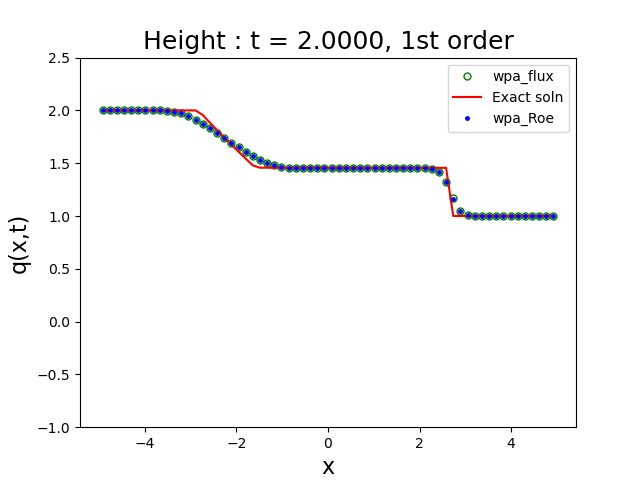
\includegraphics[width=1.0\linewidth]{images/f1}
			\caption{}
			\label{fig:f1}
		\end{subfigure}
		%
		\begin{subfigure}[b]{0.5\textwidth}
			\centering
			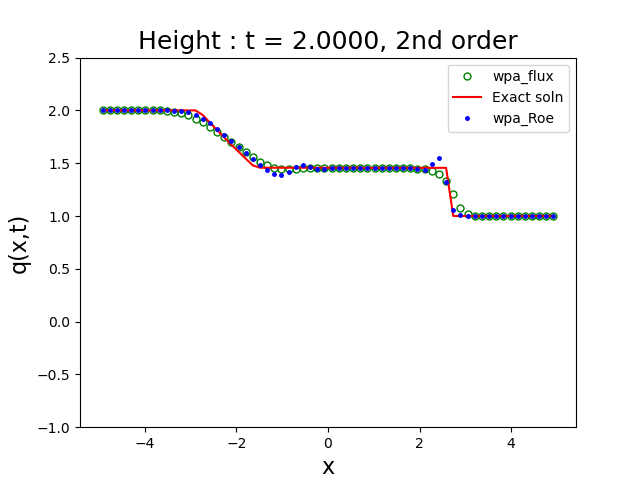
\includegraphics[width=1.0\linewidth]{images/f2}
			\caption{}
			\label{fig:f2}
		\end{subfigure}
		\caption{(a) and (b) respectively show height field at the final time step for both first and second order correction without limiters obtained after introducing the source term and the f-wave method. }
	\end{figure}
	
	  Figure.~\ref{fig:f2lim} represents Figure.~\ref{fig:f2}  with limiters used. The limiters made the Roe solver solution non oscillatory(smooth through out), and rectified the solution of the f-wave approach to replicate the jump at the 2-shock but no stationary wave was present in the solution.
	\begin{figure}[H]
		\centering
		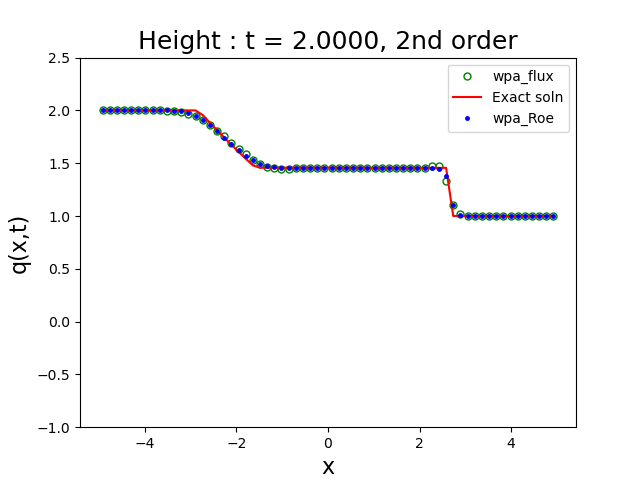
\includegraphics[width=0.5\linewidth]{images/2lim}
		\caption{Shows the height field at the final time step of second order correction with limiter obtained after introducing the source term and the f-wave method using 64 space points.}
		\label{fig:f2lim}
	\end{figure}
	\section{Riemann Problem for Wet/Dry States}
	
%\donna{Discuss importance of robust methods for handling wet/dry states (reference tsunami papers).  Reference other approaches (Toro?). Here, we describe the approach taken by George in the JCP paper. Discuss "augmented solver".}

	In the previous section we discused how the exact slover solved the Riemann problem for cases in which the water height feild id strictly positive everywhere. Dry states are regions with zero water depth. In such states SWEs are not applicable, so we consider wet states adjacent to dry regions as shown in figure~\ref{fig:dry-bed}. This enables solving SWEs in wet states, right up the boundary between wet and dry states \citep{toro2001shock}.
	\begin{figure}[H]
		\centering
		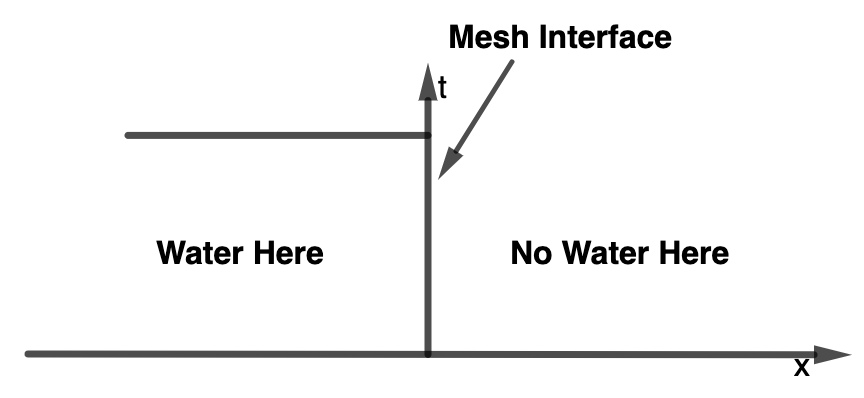
\includegraphics[width=0.5\linewidth]{images/dd1}
		\caption{ The Riemann problem with a dry bed (has no water) in one of the data state.}
		\label{fig:dry-bed}
	\end{figure}
	There are three possible cases to consider as illustrated in fig.~\ref{fig:dry-wet}. Case (a) right dry bed, the solution exhibits {\em 1-rarefaction} wave associated with the left eigenvalue $\lambda_1 = u - a$. Case (b) Left dry bed, the solution exhibits {\em 2-rarefaction} wave associated with the right eigenvalue $\lambda_2 = u + a$. Case (c) dry bed doesnot exit at $t=0$, but is created in the interaction between the two left and right wet bed regions if $S_{*L} \le S_{*R}$ where $a = \sqrt{gh}$.
	
	
	
	  
	  \begin{figure}[H]
	  	\centering
	  	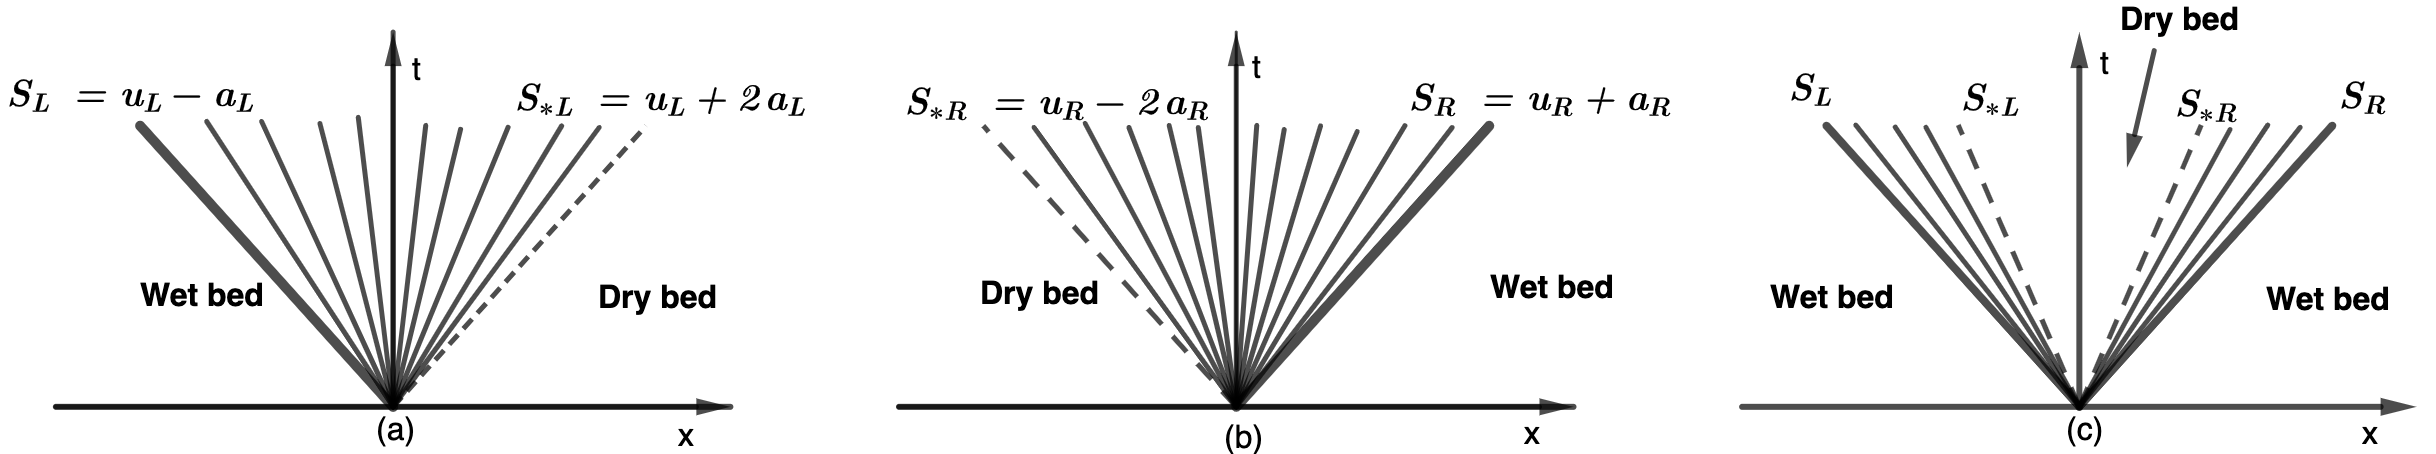
\includegraphics[width=0.7\linewidth]{images/dry-wet}
	  	\caption{The dry state appears in three cases: (a) dry region is on the right, (b) dry region is on the left, and (c) dry region appears in the interaction of two wet bed states.}
	  	\label{fig:dry-wet}
	  \end{figure}
	  
	
	  Figure~\ref{fig:right} and \ref{fig:left} respectively show solution profiles for the height field at the final time step for a Riemann problem  solved exactly with initial data containing dry bed region appears on the right and left.
	  \begin{figure}[H]
	  	\begin{subfigure}[b]{0.5\textwidth}
	  		\centering
	  		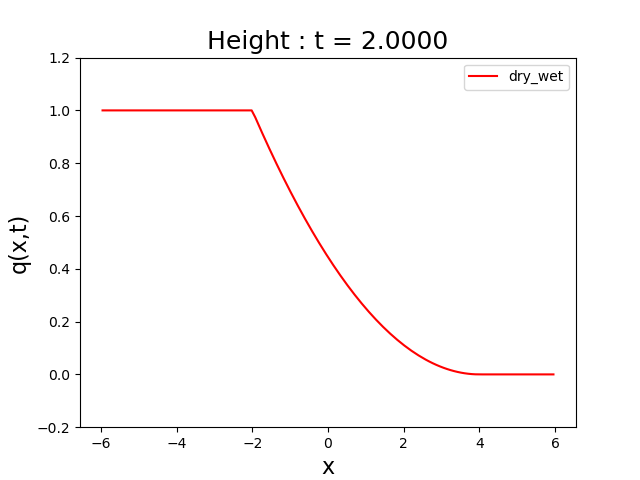
\includegraphics[width=1.0\linewidth]{images/right}
	  		\caption{}
	  		\label{fig:right}
	  	\end{subfigure}
	  	%
	  	\begin{subfigure}[b]{0.5\textwidth}
	  		\centering
	  		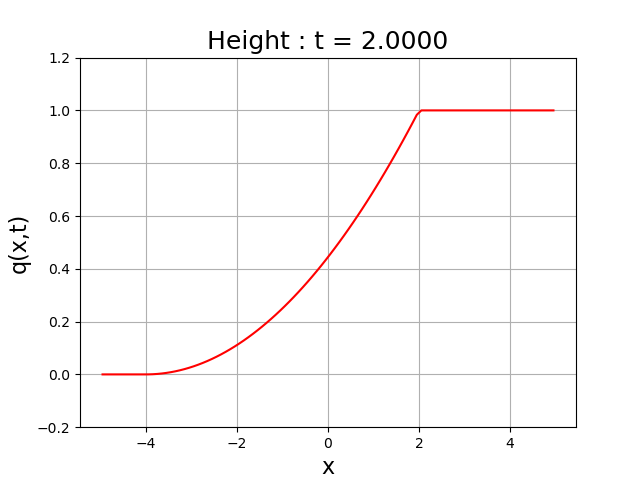
\includegraphics[width=1.0\linewidth]{images/left}
	  		\caption{}
	  		\label{fig:left}
	  	\end{subfigure}
	  	\caption{(a) and (b) respectively Shows a typical solution profile for the Riemann solution in which the dry bed is at the right and left. }
	  \end{figure}
	  Figure~\ref{fig:middle} show solution profiles for the height field at the final time step for a Riemann problem  solved exactly for which a dry bed region appears due to the interaction of two wet bed states statisfying $S_{*L} \le S_{*R}$.
\begin{figure}[H]
	\centering
	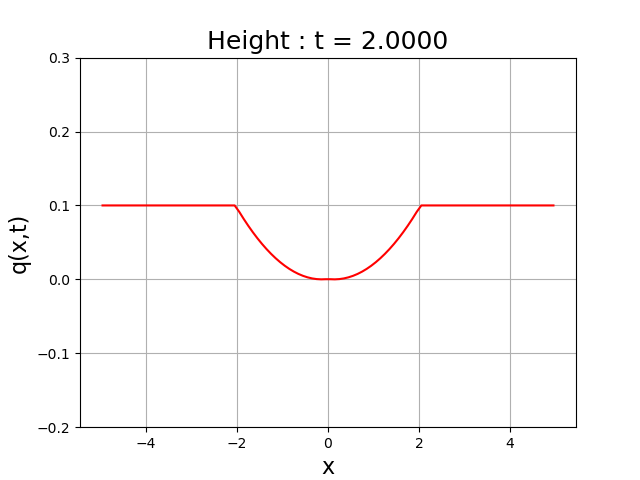
\includegraphics[width=0.8\linewidth]{images/middle}
	\caption{ Shows a typical solution profile for the Riemann solution in which the dry bed appears in the interaction between the two wet bed regions.}
	\label{fig:middle}
\end{figure}
	
	
Here, we describe the approach taken by George in the JCP paper\cite{ge:2008}. LeVeque and Pelanti in \cite{leveque2001class} proposed that equation \eqref{p3} can be decomposed into equation \eqref{p5}:
	
	\begin{equation}
		\begin{bmatrix} 
			H_{i} - H_{i-1}\\ 	HU_{i} - HU_{i-1} \\  \varphi(Q_{i}) - \varphi(Q_{i-1}) 
		\end{bmatrix} = \sum_{p=1}^{3} \alpha_{i-\frac{1}{2}}^{p} w_{i-\frac{1}{2}}^{p}
		\label{p5}
	\end{equation}
	 where the momentum flux $\varphi(q) = (hu^{2} + \frac{1}{2} gh^{2})$, $Q_{i} = (H_{i},HU_{i})^{T}$ represents the numerical solution of $q = (h,hu)^{T}$ in $C_{i}$, and $w_{i-\frac{1}{2}}^{p} \in \mathbb{R}^{3}$ ,$\forall ~ p \in [1,3] $ with $p$ a set of chosen independent vectors. \\
	
	 The decomposition of the solutions $Q_{i} - Q_{i-1} $  and  $f(Q_{i}) - f(Q_{i-1})$ $ \in  \mathbb{R}^{2}$ are represented by the first two and last two components of the three components of the decomposition \eqref{p5} respectively.  Conservation is maintained by modifying fluctuations using the last two of the three components  in equation \eqref{p5}. Then  consider $z_{i-\frac{1}{2}}^{p} \in \mathbb{R}^{2}$ for each $p \in [1,3]$ to be flux waves defined by:
	
	\begin{equation}
		z_{i-\frac{1}{2}}^{p} = [\mathbf{0}_{2\times1} \quad \mathbf{I}_{2\times2}] \alpha_{i-\frac{1}{2}}^{p} w_{i-\frac{1}{2}}^{p}
	\end{equation}
	where $\mathbf{0}_{2\times1}$ is a two by one zeros matrix, $\mathbf{I}_{2\times2}$ is a two by two identity. Then updated fluctuations become:
	\begin{eqnarray}
		\mathcal{A^{+}}\Delta Q_{i-\frac{1}{2}}^{n} = \sum_{\{ p:s_{i-\frac{1}{2}}^{p}>0\}}  z_{i-\frac{1}{2}}^{p}
		\label{p7}\\
		\mathcal{A^{-}}\Delta Q_{i+\frac{1}{2}}^{n} = \sum_{\{ p:s_{i+\frac{1}{2}}^{p}<0\}} z_{i+\frac{1}{2}}^{p}
		\label{p8}
	\end{eqnarray}
	There is only one rarefaction in the exact Riemann solution, that connects wet to dry state. The developing wet/dry interface is in this case single edge of the rarefaction, making it possible to determine the interface propagating speed using the corresponding characteristics field of the Riemann invariants \cite{ge:2008}.\\ 
	
	\noindent The wet/dry interface propagation  speed  is given by equation \eqref{wd0}, since the right state in figure \ref{fig:dry-bed}, is considered as the initial dry state, which also makes the rarefaction to be in the first characteristic field as shown in figure \ref{fig:dry-wet}.(a).
	
	\begin{equation}
		s_{i-\frac{1}{2}}^{3} = \check{s}_{i-\frac{1}{2}}^{+} = \lambda_{i-\frac{1}{2}}^{-*}(0)= U_{i-1} - 2\sqrt{gH_{i-1}}
		\label{wd0}
	\end{equation}
	
	\noindent If the left state in figure \ref{fig:dry-bed}, is considered as the initial dry state, then the  wet/dry interface propagation  speed  is given by equation \eqref{wd1}, and the  rarefaction is in the second characteristic field  as shown in figure \ref{fig:dry-wet}.(b).
	
	\begin{equation}
		s_{i-\frac{1}{2}}^{1} = \check{s}_{i-\frac{1}{2}}^{-} = \lambda_{i-\frac{1}{2}}^{+*}(0)= U_{i} - 2\sqrt{gH_{i}}
		\label{wd1}
	\end{equation}
	\section{ Future research directions}
	
	
	
	
	
	\bibliographystyle{plain}
	\bibliography{geoclaw}
	
\end{document}

